\documentclass[12pt, twosides]{report}

\usepackage{graphicx}
\graphicspath{ {figures/} }
\usepackage[left=2.5cm,right=2cm,top=2.5cm]{geometry}


\usepackage[utf8]{inputenc}
\usepackage{t1enc}
\usepackage[magyar]{babel}
\linespread{1.5}

\usepackage{footnote}
\usepackage{subfigure}
\usepackage{float}
\usepackage[]{algorithm2e}
\usepackage{amsmath}
\usepackage{mathptmx}
\usepackage{pdfpages}

\usepackage{xcolor}
\usepackage{hyperref}
\hypersetup{
    colorlinks,
    linkcolor=black,
    citecolor=black,
	urlcolor={blue!80!black},
	unicode=true
}
% 
\urlstyle{same}

\usepackage{listings}
\definecolor{dkgreen}{rgb}{0,0.6,0}
\definecolor{gray}{rgb}{0.5,0.5,0.5}
\definecolor{mauve}{rgb}{0.58,0,0.82}
\definecolor{light-gray}{gray}{0.25}

\lstdefinestyle{yaml}{	
	backgroundcolor=\color{white}, % choose the background color;
	basicstyle=\fontsize{8}{8}\ttfamily,% the size of the fonts that are used for the code
	breakatwhitespace=false, % sets if automatic breaks should only happen at whitespace
	breaklines=true, % sets automatic line breaking
	commentstyle=\color{dkgreen},  % comment style
	deletekeywords={...},  % if you want to delete keywords from the given language
	escapeinside={\%}{)},  % if you want to add LaTeX within your code
	extendedchars=true,  % lets you use non-ASCII characters; for 8-bits encodings only, does not work with UTF-8
	frame=none,	 	 % adds a frame around the code
	keepspaces=true, % keeps spaces in text, useful for keeping indentation of code (possibly needs columns=flexible)
	keywordstyle=\color{blue}\bfseries, % keyword style
	otherkeywords={*,...}, % if you want to add more keywords to the set
	numbers=none,  % where to put the line-numbers; possible values are (none, left, right)
	numbersep=5pt, % how far the line-numbers are from the code
	numberstyle=\tiny\color{gray}, % the style that is used for the line-numbers
	rulecolor=\color{black}, % if not set, the frame-color may be changed on line-breaks within not-black text (e.g. comments (green here))
	showspaces=false,% show spaces everywhere adding particular underscores; it overrides 'showstringspaces'
	showstringspaces=false,  % underline spaces within strings only
	showtabs=false,  % show tabs within strings adding particular underscores
	%stepnumber=1,  % the step between two line-numbers. If it's 1, each line will be numbered
	stringstyle=\color{mauve}, % string literal style
	tabsize=2,
	columns=fullflexible  % Using fixed column width (for e.g. nice alignment)
	sensitive = true,
	morekeywords={name, runs-on, on, jobs, build, run, steps, uses}
}
\lstset{style=yaml}

\title{
	{Price-Monitor}\\
	{\large Sapientia\\
	Erdélyi Magyar Tudományegyetem, Marosvásárhely}
}
\author{
	Palfi Szabolcs\\
	\texttt{palfi.szabolcs@student.ms.sapientia.ro}
	\and
	Szántó, Zoltán\\
	\texttt{zoltan.szanto@ms.sapientia.ro}	
}
\date{2021}

%%%%%%%%%%%%%%%%%%%%%%%%%%%%%%%%%%%%%%%%%%%%%%%%%%%%%%%%%%%%%%%%%%%%%%%%%
\begin{document}


\includepdf[pages={1,2,3}]{pdfs/allamvizsga_borito.pdf}

\section*{Extras}
În zilele noastre, majoritatea cumpărăturilor se fac online. Sunt foarte multe magazine online, care iți promit diferite promoții, indiferent de perioada anului. Aceste promoții de multe ori sunt doar de fațadă, în spatele lor de fapt nu este nici o scădere reală de preț. Aceste aspecte se pot observa doar în cazul în care urmărim prețul unui produs zilnic, ceea ce este foarte repetitiv și solicitant față de timpul nostru. Toate aceste aspecte sunt valabile și în cazul în care dorim să cumpăram produsele la prețuri corecte și cu adevărat aflate la promoție. 

In această lucrare este prezentat un sistem pentru monitorizarea prețurilor care automatizează procesul descris mai devreme. Sistemul se trezește in momente predefinite pentru a mina date publice de pe Internet, care apoi vor fi salvate. Utilizatorul are la dispoziție o extensie de browser și o aplicație pentru telefon realizată in Flutter, prin care poate adăuga produse noi în lista lui și poate urmări pe un grafic, evoluția preturilor. Așa zisa inimă a sistemului o reprezintă un script realizat în Python, care este responsabil pentru adunarea datelor, actualizarea periodică a prețurilor și a adăugării unor noi produse în lista utilizatorului. Datele adunate sunt stocate într-o bază de date furnizată de Firebase, care s-a dovedit a fi ideală în utilizarea noastră. 

După luni de adunare a datelor, folosind sistemul implementat, am analizat datele, după care am făcut câteva observații interesante. Au fost mai multe modele după care se schimbau preturile, însă nu a fost niciunul concludent și valabil pentru toate produsele. Au fost mai multe cazuri unde am observat manipulări ale prețurilor, mai ales in perioada de Black Friday, dar pe de altă parte am observat și prețuri cu promoții reale și semnificative așa că este destul de greu de generalizat în acest sens. După folosirea îndelungată a software-ului putem concluziona că acesta poate fi de folos unui potențial cumpărător, prin furnizarea unor informații utile și într-o formă ușor de citit, astfel economisind și timp. 

\textbf{Cuvinte cheie}: webscraping, extensie de browser, aplicație Flutter
\pagebreak


\includepdf[pages={6}]{pdfs/allamvizsga_borito.pdf}

\section*{Kivonat}
Napjainkban az emberek nagy többsége a vásárlásaikat az online térben bonyolítják le. Rengeteg webáruház létezik, szinte állandóan vannak kedvezmenyék vagy ajánlatok. Viszont sok esetben a feltüntetett árak ingadoznak, vagy a kedvezmény csak látszólagos. Ezekre akkor lehet felfigyelni, ha napi szinten követjük az árak alakulását, viszont ez időigényes és repetitív folyamat. Ugyanez elmondható akkor is, ha egy terméket megszeretnénk vásárolni kedvező áron. Egy másik népszerű online áruházakkal kapcsolatos jelenség a Black Friday napján történő drasztikus árcsökkentés, vagy legalábbis annak a látszata, hiszen sokszor hallottuk vagy gondoltuk, hogy ezek igazából hamisak vagy a csökkenés mértéke jóval kisebb, mint az valójában fel van tüntetve. Ezen gondolatok szolgálták a rendszer megvalósításához szükséges inspirációt.

A dolgozatban bemutatunk egy árakat követő rendszert, mely az előbb említett napi ellenőrzés folyamatát automatizálja. A rendszer meghatározott idő pillanatokban felébred, az online web áruházakon elérhető publikus adatokat bányássza, és az eredményeket elmenti. A rendszer biztosit egy böngésző kiegészítőt a termékek hozzáadására, követésére, illetve egy egyéb műveletekre. A mobil alkalmazás ugyanazt a funkcionalitást biztosítja, mint a böngésző kiegészítő, ez Flutter segítségével lett megvalósítva. A szoftver szívét úgymond egy Python script biztosítja, amely az adatok bányászását végzi a követni kívánt weboldalakról, valamint a periodikus frissítésért is felelős. Természetesen ezek az modszerek minden morális, illetve jogi feltételnek eleget tesznek a bányászás során. A bányászott adatok a Firebase által szolgáltatott Realtime Database segítségével vannak eltárolva, ami rendkívül jó és megbízható platformnak bizonyult a jelen felhasználásra.

A hónapokon keresztül gyűjtött adatokat kielemezve le tudtunk vonni pár következtetést éspedig azt, hogy valóban valamilyen szinten manipulálva vannak az árak, hiszen több érdekes mintára is felfigyeltünk, viszont ezek nem minden esetben a vásárló becsapását jelentik, volt példa reális és igencsak jelentős árcsökkenésre is, ezért eléggé nehéz általánosítani. A rendszer hosszabb idejű használata során az a következtetés vonódott le, hogy igencsak hasznos lehet egy ilyen jellegű szoftver a vásárlok számára, hiszen valamilyen mértékben könnyebbé teheti a döntési folyamatot, az információk összesítése és ábrázolása által.

\textbf{Kulcsszavak}: webscraping, böngésző kiegészítő, Flutter alkalmazás
\pagebreak

\section*{Abstract}
These days the majority of shopping is done online. There are tons of online shopping websites, with some kind of big sale going on almost all the time, however these sales are most of the time made up. These false sales can be spotted only if you follow a products price daily, for a longer period of time which is a repetitive and time-consuming process. The same can be said when you’re interested in purchasing some products but you’re not quite decided yet, so you want to wait for the price to drop. These gave the inspiration for developing our system.

In this paper we’ll present a price monitoring system which automates the process described earlier. At predefined moments the system wakes up and scrapes publicly available data from the Internet, which are than saved. The user has the opportunity to add products to his list, for them to be followed, and can view the price change on a chart. All this can be done from a Chrome browser extension or a mobile application built with Flutter. The so-called heart of the system is a python script which is responsible for the mining of the data, periodically updating the prices and pushing new products into the database. All this is done while respecting all moral and legal boundaries. All of our data is stored in a Realtime Database provided by Firebase, which turned out to be perfect for our application.

After months of gathering data, while using the system, we analyzed it and made a few conclusions. We saw multiple patterns emerging from the price changes but there is not one that matches every product. There were many scams regarding prices, especially during Black Friday but there were also real and significant price drops as well. After using the system for a longer period of time we can say that a software like this helps the buyers in making a purchase decision, by providing useful data in a easy to read form.

\textbf{Keywords}: webscraping, browser extension, Flutter app
\pagebreak

\pagenumbering{gobble}

\tableofcontents

\listoffigures

\chapter{Bevezető}
\pagenumbering{arabic}
A mai rohanó világban a bevásárlások egyre növekvő százaléka történik Interneten, mindez lehetőséget nyújtva a vásárlóknak, hogy egy bizonyos terméket több, akár hazai akár külföldi, oldalról is megvásárolhasson. Az e-commerce-el foglalkozó cégek rohamos fejlődésnek indultak az utóbbi évtizedben mely maga után vonja az érdekesebbnél érdekesebb marketing fogásokat, melyekkel a célközönséget próbálják vásárlásra bírni.

Valószínűleg mindenki hallott már a “Black Friday” az-az „Fekete Péntek” -nek nevezett jelenségről amely inspirációként szolgált az alkalmazás megvalósításához. Ez a kifejezés legelőszőr az 1800-as években fogalmazódott meg, amikor is Jay Gould és James Fisk az amerikai arany árak manipulálása által 20\%-os esést okoztak a részvénypiacon melynek következtében az árucikkek értéke felére csökkent \footnote{\url{https://en.wikipedia.org/wiki/Black_Friday_(1869)}}. A 20. század közepe fele ez már egészen más jelentéssel bírt, ugyanis a Hálaadás ünnepét követő napon, az-az pénteken vette kezdetét a karácsonyi árleszállítás, mely sok cég esetében életmentő volt, hiszen ekkor kerültek át a veszteséges állapotból melyet pirossal jelöltek, a jövedelmezőbe, amit már fekete írószerrel jegyeztek fel \footnote{\url{https://en.wikipedia.org/wiki/Black_Friday_(shopping)}}. Ebben az időszakban a megszokottnál jóval nagyobb és több árleszállítással vonzották az embereket.

Mint azt sokan tudjuk, országunkban is nagy népszerűségnek örvend ez a jelenség, habár eléggé távol áll az eredeti koncepciótól. Nagyon sok mesterséges árleszállítással próbálják becsapni az embert, melyet legtöbb esetben jól kitervelt áringadozással oldanak meg\footnote{\url{https://cavaleria.ro/tepele-de-black-friday-2020/}}. Ugyanakkor, nem kizárólag ebben a periódusban lehet észrevenni az úgymond „hamis” kedvezményeket ezért szükségét láttuk egy olyan alkalmazás kifejlesztésének, amely nyomon tudja követni egy megadott termék árat, illetve annak ingadozását.

Mivel az Interneten publikus adatok találhatók, ezek felhasználásával semmiféle kár nem keletkezik az adott weboldalak számára. Egy internetes oldal betöltése során, mi, mint felhasználók, egy kérést intézünk egy szerver fele a böngészőnkön keresztül, ami majd a kapott válasz alapján felépíti és megjeleníti számunkra a megtekinteni kívánt oldalt. Ezt a műveletet természetesen legtöbbször ahogy az előbbiekben is említettem, böngészőn keresztül végezzük, viszont ez nem egy szükséglet, inkább egy eszköz, számos más módon is intézhetünk kéréseket egy adott szerver fele. Az általunk megvalósítani kívánt alkalmazás ezt a tulajdonságot hivatott kihasználni, ezáltal nyilvánosan elérhető adatok begyűjtésével, feldolgozásával és elemzésével szeretne foglalkozni.


\chapter{Célkitűzések}
Az alábbi fejezetben összefoglaljuk az alkalmazás fontosabb célkitűzéseit. A fő cél, mely érdekében létrejön a szoftver, az, hogy segítsen egy potenciális vásárlónak követni egy adott termék arának időbeli változását. Ennek megfelelően, a következő célok fogalmazódtak meg:
\begin{itemize}
    \item Rövid használati útmutató, szöveges formában
    \item Támogatott oldalak listázása
    \item Regisztrálási, bejelentkezési lehetőség biztosítása, hogy különböző eszközökön is, mint például mobilos vagy webes, elérhetőek legyenek a követett termékek információi
    \item Felhasználói fiók jelszavának változtatási lehetősége, felhasználói fiókból való ki jelentkezés valamint annak törlése.
    \item A termékek ábrázolása listaszerűen történjen
    \item Az árak változását a felhasználó számára grafikus formában szeretnénk ábrázolni a könnyebb átláthatóság érdekében
    \item Az árak időben való változását könnyen átlátható vonal diagramon ábrázolni
    \item Egyszerű átirányítás a termék oldalára
    \item Telefonos alkalmazás
	\item Kiegészítő, Chrome alapú böngészőkre
\end{itemize}

\chapter{Szakirodalom áttekintése ? Technologiai áttekintés}
\section{Web bányászat}

Web bányászat, vagy angol kifejezésben Web mining, alatt azt a folyamatot értjük, amely által új, eddig nem ismert, de hasznos információt fedezünk fel az Interneten található adatok között. Mindezt a cégek arra használják, hogy új értékes információkat gyűjtsenek, ezeket feldolgozzák, majd ezek által a felhasználókat vagy fogyasztókat jobban megismerjék. Ez a folyamat az úgynevezett adat bányászat technikát alkalmazza ahhoz, hogy automatikusan kinyerje az adatokat az Internetről \cite{gorunescu2011data}. 

Számos más technikát is alkalmaztak már új információk kinyerésére, az így is hatalmas és egyre növekvő adat mennyiségből, mint például az Information retrieval, Information extraction illetve gépi tanulás. Az Information retrival működési elve az, hogy a szöveg indexelésé után nyeri ki a hasznos információt. Az Information Extraction arra fokuszál, hogy csak a lényeges információt nyerje ki, míg az előbb említett inkább hasznos dokumentumokat jelöl meg. A gépi tanulásos módszer nem kötődik direkt módon a Web Scraping-el viszont segítséget nyújt a szövegek osztályozási folyamatában. A web bányászatot három fő kategóriába soroljuk, ahogy az látható az \ref{fig:web_mining_rendszertana} ábrán is.

\begin{figure}[h]
    \centering
    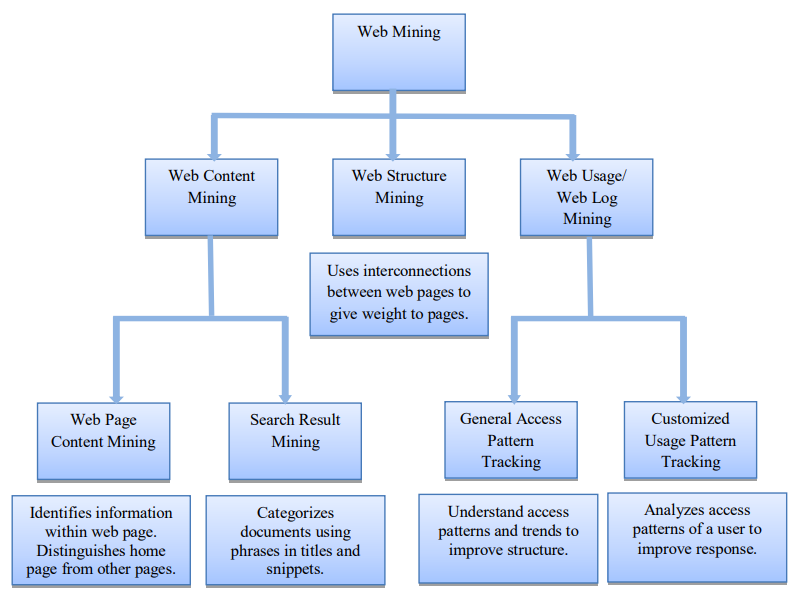
\includegraphics[scale=1, width=\textwidth]{figures/images/web_mining_rendszertan.png}
    \caption{A Web Bányászat rendszertana \cite{johnson2012web}}
    \label{fig:web_mining_rendszertana}
\end{figure}

A Web Content Mining vagy magyarul webes tartalom bányászat, olyan tartalmakra fekteti a hangsúlyt, mint például szöveg, kép, audió, videó, metaadatok, hiperlinkek. Ezek tanulmányozása, segít nekünk megérteni a felhasználók, vásárlók viselkedését mely által a weboldalak teljesítményét növelni lehet a későbbiekben, hogy azok jobban, illetve hatékonyabban működjenek. 

Mivel a webes tartalom bányászat megvizsgálja úgy a kereséseket, mint azoknak a konkrét tartalmát ezért ezt is tovább lehet osztani két kategóriába, Keresési Eredmény, illetve Weboldal Tartalom bányászat. Nevükből adódóan, ezek kiegészítik egymást, mivel a tartalom bányászat azon oldalakon történik, melyeket korábban megvizsgált és ígéretesnek talált a Keresési eredmény általi elemzés. A Web Structure Mining egy olyan ágazat, mely struktúrák bányászásával foglalkozik, mint például HTML vagy XML címkék, amely által weboldalak közötti kapcsolatot tud felismerni, ezáltal súlyokat rendelve azokhoz. A Web Usage Mining által lehet megérteni a különböző használati mintákat, amelyeket a felhasználók követnek, ezeket főként naplózás, felhasználók profiljai, sütik, könyvjelzők által, de ugyanide tartoznak a különböző egér mozdulatok vagy görgetési adatok is.

\section{Web Struktúra bányászat}

Rengeteg új adat generálódik az Interneten, napról napra az adat mennyiség exponenciálisán növekszik. Bőségesen állnak rendelkezésünkre szolgáltatások, illetve információk, elektronikus áruházak, elektronikus újságok, közösségi oldalak formájában, hogy csak párat említsünk. Habár ezen adatok fogyasztás céljára lettek szánva, sok időt el lehet tölteni az adatok kinyerésével és elemzésével. Továbbá, a weboldalak adatai HTML, illetve más webre szánt formátumban vannak jelen, amely megnehezíti az automata feldolgozást. Ez lett a mozgató rugója az ezen a téren zajló kutatásnak, mint például a Web Scraping.

A Web Structure Mining, vagy ismertebb nevén Web Scraping, az a folyamat, amely által hasznos információkat nyerünk ki egy weboldal HTML kódjából, amely az Internet fő formázási eszköze \cite{dastidar2016intelligent}. Az egyik metodológia megállapította, a rendezett annotációk, melyek nem mások, mint gépek számára is értelmezhető leíró információk az adott oldalra tekintve, egy külön szemantikus rétegben vannak tárolva, elválasztva a weboldaltól, ezáltal megkönnyítve és felgyorsítva a bányászási folyamatot, mivel először ezeket a fontos metaadatokat dolgozza fel, majd csak ezt követően magát a weboldalt.

A HTML struktúráját tekintve, két fő adat típust lehet bányászni belőle. Az egyik a felhasználó által generált - a másik pedig a metaadat. A felhasználó által generált adat bármi olyan típusú adatra vonatkozik, amelyet a felhasználó hozott létre vagy adott hozzá a weboldalhoz, akár személyesen akár egy közösségi platform hozzácsatolásával. A metaadat definíció szerint olyan adat, amely leír egy másik adatot \cite{landers2016primer}, ezek általában minden weboldalon megtalálhatók, fontosabb leíró adatokat tartalmazva, mint például szerző, cím, cikkek eseten megjelenés időpontja, kulcsszavak. Ezek általában nem láthatóak a felhasználó számára, viszont kiolvashatóak az adott oldal HTML kódjából \cite{landers2016primer}.

\subsection{Személyre szabott információ lekérése példával illusztrálva}

Tegyük fel, hogy egy személy fárasztónak találja, hogy a nap végen a fontos vagy számára értékes hírek után keressen, vagy előkeresse a kedvenc sport csapata elért eredményeit. Egy intelligens Web Scraper a tökéletes eszköz ebben az esetben, mivel az időközönként végig tudja böngészni az Internetet a felhasználó által megszabott témakörökben található információk után kutatva, vagy akár specifikus kulcsszavakat tartalmazó híreket előkerítve. Ez egy előre weboldalakat tartalmazó listán menne végig, melyet a felhasználó határoz meg, hogy a számára hiteles információt kapja meg \cite{dastidar2016intelligent}.

Egy másik példa egy Web Scraper felhasználására az, amikor például egy vásárló több terméket is kinézett magának, több különböző weboldalon. Ha esetleg nem szeretné azonnal megvásárolni a terméket, hanem csak követni annak árát, akkor esettől függően, több oldalra is be kell jelentkeznie, több felhasználóval oldalankent, de legjobb esetben is számos oldalt kellene naponta megfigyeljen és lejegyezzen. Egy Web Scraper abban könnyítené meg a felhasználó dolgát, hogy például egy böngészős kiegészítő keretein belül, a vásárló hozzá tudja adni egy listához a terméket és attól a pillanattól, a program naponta akár többször is le tudja kérni a termék árát, anélkül, hogy a felhasználó bármit is tenne. Ezáltal egy helyen lenne a vásárló több terméke, és pár kattintással tisztább kepét alkothat a termékek árára vonatkozóan.

\section{Web Scraping gyakori alkalmazásai}

A web scrapinget, adatgyűjtő jellege miatt számos területen fel lehet használni, illetve igénynek megfelelően alakítani. Ezekre pár példa:

\begin{itemize}
    \item Online ár összehasonlítás – ugyanazon termék arának összehasonlítása több weboldalon, pl. https://www.compari.ro/, https://www.price.ro/ 
	\item Contact Scraping – általában email címeket gyűjtenek, marketing céljából
    \item Időjárással kapcsolatos adatok gyűjtése
    \item Weboldal változásainak figyelése
	\item Több forrásból származó adat egyesítése
	\item Kedvezmény kuponok pl. pouch – chrome extension
	\item Álláshirdetések összesítése
	\item Brand monitoring – egy bizonyos márkához tartozó adatokat gyűjtik, általában az ahhoz társított véleményre kíváncsiak
    \item Piac tanulmány – egy adott termék piacon való elhelyezkedését, illetve potenciális sikerességet próbáljak megjósolni a bányászott adatok átvizsgálásával.
\end{itemize}

\section{Web Scraping módszerek}
Számos technika áll rendelkezésünkre melyekkel az adatgyűjtést végezhetjük, ezeket mindig az adott helyzetnek megfelelően kell kiválasztani, főként a hatékonyságot tartva szemelőt. Ebben a részben a Web Scraping egy pár technikája kerül röviden ismertetésre.

\begin{itemize}
\item Copy-paste - Időközönként valaki kézzel történő adatgyűjtést, valamint vizsgálatot végez. Adott helyzetekben ez a leghatékonyabb módszer, viszont nagyon hajlamos a hibákra, sok időt és fáradságot vesz igénybe az ember részéről, amíg a nagy adathalmazokat feldolgozza.
\item Reguláris kifejezések - Ez egy egyszerű és erőteljes megközelítése az információ gyűjtésnek. A UNIX vagy más programozási nyelv által használt reguláris kifejezés illesztésen alapszik.
\item HTML Parsing – Félig strukturált lekérdező nyelvek segítségével elemezni, illetve módosítani a weboldalak tartalmát.
\item DOM Parsing – A böngészőkbe beépített kezelő programok segítségével, az erre a célra fejlesztett alkalmazások lekérhetik a kliens oldalon dinamikusan létrejött tartalmakat is, mellyel utána fel tudják építeni a DOM fát, ebben pedig könnyebben lehet specifikus adatok után keresni.
\item Web Scraping Szoftver – Számos szoftver áll rendelkezésünkre, amelyeket személyre szabott keresésre lehet használni. 
\item Mesterséges Intelligencia – Több helyen is kísérleteznek gépi tanulásos adatbányászattal, melynek az a célja, hogy a gépek megtanulják úgy értelmezni a weboldalakat, ahogy azt az emberek tennék.
\end{itemize}

\section{Web Scraping szoftverek}
Több szoftver is rendelkezésünkre áll a piacon, úgy ingyenes mint fizetett formában is, mindegyiknek megvan az erőssége illetve, gyengesége, ezek közül egy párat mutat be a jelen fejezet. 

\begin{itemize}
\item A Web Scraping szoftverek rendkívül fontos szerepet játszanak ezen a téren, mivel automatizálják és rendkívül felgyorsítják az adat-gyűjtő, valamint feldolgozó folyamatot. Számos ilyen szoftver található a piacon, a maga előnyeivel és hátrányaival. Ezeknek az ára a funkcionalitásuk függvényében, valamint a támogatás és frissítési időszakok függvényében változik. 
\item Visual Web Ripper\footnote{\url{http://visualwebripper.com/}} – Az egyik legfejletteb web scraping szoftver, melyet a Sequentum csoport fejlesztett 2006-tól kezdődően. Weboldalakról gyűjtött információk bányászására használják, úgy egyszerű weboldalak, mint e-commerce oldalak esetében, mint például eBay, Amazon, magento, azonban titkosított tartalmak eseteben is segítségünkre lehet. A bányászott adatokat kimenthetjük adatbázisba vagy CSV, illetve XML formátumban is. Előnye, hogy vizuális felülettel rendelkezik, ezért rendkívül egyszerűen ki lehet választani, hogy pontosan mit is szeretnénk. Egyszeri fizetéssel lehet megvásárolni a szoftvert, \$349.00 áron\footnote{\label{price_disclaimer}Az árak aktualitásáért lásd a szolgáltató weboldalát}, viszont fontos szempont, hogy ezen alkalmazás elveszti a gyártó általi támogatottságát 2021-gyel kezdődően, kivételt kepézve azon esetek, ahol a vásárlóval karbantartási szerződés van érvényben, mely túlhaladja ezt az időpontot.
\item Web Content Extractor\footnote{\url{https://www.webcontentextractor.com/}} – Nagyon jó automatizálási lehetőséget nyújt, rendkívül egyszerűen használható, pár kattintással meg lehet adni a kivánt mintát, ami szerint majd adatokat fog gyűjteni. A program rugalmas, abból a szempontból, hogy nem próbálja túlokoskodni a felhasználót, hanem egy előlnézetet ad az eredményről, majd a felhasználó maga végezheti el a szükséges módosításokat, amennyiben szükség van erre. Ezt a szoftvert, bérlet alapú előfizetéssel lehet megszerezni, több változat is elérhető, az árak \$30 - \$150 / hónap\footref{price_disclaimer} között mozognak.
\item Mozenda\footnote{\url{https://www.mozenda.com/}} – Az egyik legegyszerűbben használható szoftver ezen a téren, ami lehetővé teszi a kevésbé technikailag hozzáértő személyeknek is, az egyszerű bányászásokat. Fő különbsége más alkalmazásokhoz kepést, hogy maga az adatbányászati folyamat a felhőben történik és nem a felhasználó erőforrásait felhasználva, amely hatalmas előnyt jelenthet. Elérhető egy 30 napos próba csomag is, ami után \$250/hónap-tól\footref{price_disclaimer} kezdődően változnak az árak, a választott csomag függvényében.
\item Screen-Scraper\footnote{\url{https://www.screen-scraper.com/}} – Nagyon fejlett web scraping alkalmazás, amelyet több változatban is el lehet érni. Az alapszínűt verzió ingyenes, ezzel egyszerűbb adatok után lehet bányászni, könnyen kezelhető, nem kell sok technikai tudás hozzá. Más változatok, mint például a profi vagy vállalkozás szintű verziók már sokkal komplexebbek, több lehetőséget nyújtanak. Nagy előnyé, hogy más rendszerekkel könnyen összeférhető pl. Java, ezért fel lehet használni más, nagyobb szintű programokban is.
\end{itemize}

Természetesen sok más program is rendelkezésünkre áll, melyek hasonló funkcionalitásokkal rendelkeznek, minden esetben az adott alkalmazásnak megfelelőt és legjobban illőt érdemes választani a nagyobb hatékonyság érdekében. Egyéb web scraper szoftverek \cite{sirisuriya2015comparative}: WebHarvy, Easy Web Extract, WebSunDew, FMiner, Scrapy, import io. 

\section{Legális és Etikai keretek}

Ebben a fejezetben a legális valamit etikai kérdésekről lesz szó, amely elég megosztó, illetve nem teljesen egyértelmű terület. Egyenesen a Web Scraping-et nem szabályozza semmilyen törvény, de több területen is problémába lehet ütközni, ilyen például a védett tartalom, az úgynevezett szerződésszegés vagy GDPR. Attól függően, hogy a bányászat milyen országhoz tartozó területen zajlik, figyelembe kell venni az ottani törvénykezést is, ezért is nehéz konkrétan jellemezni legalitási szempontból. A legpontosabb jellemzés talán az lenne, hogy van, ami igen és van, ami nem.

\subsection{Felhasználói feltételek}

Ugyanúgy, mint egy szoftver vagy szolgáltatás esetén, amikor egy weboldalt használunk el kell fogadnunk bizonyos felhasználói feltételeket, melyek leggyakrabban kis felrúgó ablakkent jelennek meg, amikor először látogatunk a weboldalra, vagy ezeket a regisztrálás folyamán tudatosítják velünk. Amennyiben valamilyen módon megszegjük ezeket a feltételeket, érvénybe lép a fentebb említett szerződésszegés. Mivel ez csak akkor érvényes, ha a felhasználó explicit módon elfogadja a feltételeket, ezért jogi szempontból nehéz kizárni a Web Scrapinget \footnote{\url{https://www.todaysoftmag.ro/article/3246/consideratii-legale-si-etice-in-contextul-scalarii-procesului-de-web-scraping}}. 

\subsection{Szerzői jogok}

Bányászni vagy újra publikálni olyan adatokat vagy információkat, amelyeknek a szerzője explicit módon fenntartja a szerzői jogokat, legális szempontból szerzői jogsértésnek minősül. Ugyanakkor egy weboldal nem minden esetben rendelkezik a felhasználói által generált adatokkal, vegyünk példának egy film értékelő oldalt, ahol a felhasználók kifejtik a véleményüket \cite{krotov2018legality}. Más ebbe a kategóriába tartozó tartalmak például a videók, kepék, zenék, adatbázisok, cikkek. Maga a bányászása ezeknek az adatoknak nem teszi illegálissá, a felhasználási módjuk határozza meg azt, hogy milyen kategóriába soroljuk azt. Az hogy milyen adatokra hogyan vonatkoznak ezek a szabályok országonként változik, van ami egyes országokban megengedett másokban viszont nem.

\subsection{GDPR}

Az Európai Unió által érvénybe léptetett Általános Adatvédelmi Rendelet\footnote{\url{https://gdpr-info.eu/}} alapján nem tiltott az adatbányászat, kivételt kepézve, ha ez a tevekénység nem tartalmaz személyes adatokat. Ilyennek minősül a név, lakcím, email cím, telefonszám, bankkártya adatok, banki adatok, IP cím, születési dátum, foglalkoztatási információk, orvosi adatok, személyes fotók vagy videók.

Ugyanakkor, mint minden más esetben itt is figyelembe kell venni az országok törvényei és szabályozásait ilyen értelemben. Mint sok más országban, Romániában is csak homályos úgy a törvénykezés mint az alkalmazási metodológia is, például nem világos hogy egy román ip címről mit bányászatunk egy kanadai oldalról és így tovább. 
\subsection{Weboldal károsítása}

Ha bármilyen tevekénység által, amelyet a Web Scraper végez, túlterheljük az adott weboldal szervereit vagy bármilyen módon sértjük, gátoljuk annak működését bűncselekménynek számít és legális következményei lehetnek. Ehhez azonban a kárnak anyaginak kell lennie, valamint könnyen bizonyíthatónak bíróság elött, ahhoz, hogy bármiféle kártérítési kérelemre legyen jogosult a weboldal \cite{krotov2018legality}. 

A fentieket figyelembe véve tehát, nem lehet egyértelmű választ adni arra, hogy a Web Scraping legális-e vagy sem. Helyette a válasz az, hogy helyzettől függ. Maga a Web Scraping nem illegális, viszont akár az is lehet a következő három dolog függvényében \cite{isWSLegal}. 

\begin{itemize}
    \item Hogyan lett bányászva az adat?
    \item A bányászott adat típusa
    \item Hogyan lesz felhasználva a bányászott adat?
\end{itemize}

Ahhoz, hogy eldöntsük az esetünk legalitását meg kell vizsgálni, hogy az adat, amit szeretnénk bányászni publikusan elérhető-e vagy sem. Ha az adat eléréséhez nem szükséges bejelentkezni egy adott oldalra akkor a felhasználói feltételek nem érvényesek ezért legálisan lehet bányászni, mivel ez az adat publikusnak számít. Ha bejelentkezésre van szükség a bányászni kívánt adat eléréséhez, akkor a felhasználói feltételek tanulmányozásával el kell dönteni, hogy legális-e vagy sem, mivel azok elfogadásával legálisan alkalmazhatóvá vált számunkra, azaz a megszegésük jogi következményeket vonhat maga után.

A bányászott adat típusa szerint két formájára kell nagyon odafigyelni, Személyes Adatok és Szerzői Jogokkal rendelkező adatok, ezek fentebb részletesebben is tárgyalva voltak.

Az adatok felhasználása során figyelembe kell venni, hogy az illegális módon vagy csalás által történő adatgyűjtést minden állam bünteti, tehát ez bűncselekménynek minősül. Amennyiben olyan tartalmakat bányászunk melyek bizalmas vagy bármi féle módon védett információt tartalmaznak, ezeknek felhasználása ugyancsak törvényszegést jelent és az erényben levő büntető eljárások érvényesek. Természetesen, legtöbb esetben már maga az törvénysértő lehet, hogy ezekhez az adatokhoz jogosultság nélkül fértünk hozzá, ezért egyértelműen nem felhasználhatóak ezek az adatok. 

Leegyszerűsítve, három alapvető kérdésre kell választ adni, ahhoz, hogy eldöntsük legális-e az adat bányászat, amelyet végre szeretnénk hajtani: 

\begin{itemize}
    \item Bejelentkezés által elérhető adatot bányászok?
    \item Személyes adatot bányászok?
    \item Szerzői jogokkal rendelkező adatot bányászok?
\end{itemize}

Amennyiben mindhárom kérdésre nemleges a válasz, legálisnak bizonyul adott esetben a Web Scraping. Azonban, ha bármelyik kérdésre pozitív választ adunk nagy valószínűséggel újra kell gondolni és figyelmesebben megvizsgálni az eset legális mivoltát. Ugyanakkor egyik esetben sem szabad megfeledkezni arról, hogy minden ország másképp kezelheti ezen kérdéseket, ezért ilyen értelemben is vizsgálódnunk kell.

% \chapter{Elméleti áttekintés}
% \section{Elméleti áttekintés}

Pszeudokód: 

\begin{algorithm}[h]
    \begin{small}
    \KwData{Tanulási tényező ($\alpha \in (0, 1])$), $\epsilon > 0$}
    Véletlenszerű érték minden $Q_{1}(s,a)$ és $Q_{2}(s,a)$-nek, kivéve $Q($terminális$, \cdot ) = 0$, $s \in S$, $a \in A$ \;
    \For{minden epizód}{
        S inicalizálása\;
        \Repeat{S terminális állapot}{
        $A \leftarrow$ cselekvés, $S$ állapotban $\epsilon$-greedy szerint $Q_{1}+Q_{2}$ \;
        $A$ cselekedet végrehajtása, R és S' megfigyelése\;
        \eIf{ $50\%$ eséllyel}
            {$Q_{1}(S, A) \leftarrow Q_{1}(S, A) + \alpha [R + \gamma Q_{2}(S', arg\max_{a}Q_{1}(S', a)) - Q_{1}(S, A)]$}
            {$Q_{2}(S, A) \leftarrow Q_{2}(S, A) + \alpha [R + \gamma Q_{1}(S', arg\max_{a}Q_{2}(S', a)) - Q_{2}(S, A)]$}
        $S \leftarrow S'$\;
        }
    }
    \end{small}
    \caption{Dupla Q-tanulás \cite{sutton2018reinforcement}.}        
    \label{algo:double_q}
\end{algorithm}


Hivatkozás pszeudokódra: \ref{algo:double_q}.

\chapter{Rendszer specifikációi}
\section{Felhasználói Követelmények}

A felhasználónak mindenekelőtt be kell tudnia jelentkezni, ahhoz, hogy elérje a terméklistáját, ez azért fontos, mivel eszköz váltás esetén nem szeretnénk elveszíteni az addig követett termékeket. A bejelentkezéshez szükséges adatok a regisztrációkor megadott email cím, illetve jelszó. Mindezt az \ref{fig:login_activity_diag} ábra illusztrálja. A felhasználó jelszava base64 hash általi titkosítással van eltárolva, ezáltal az nem elérhető eredeti formájában, ezt a funkciót a bejelentkezést megvalósító Firebase Authentication valósítja meg, amely jelszó módosítási lehetőséget is lehetővé tesz.

\begin{figure}[h]
    \centering
    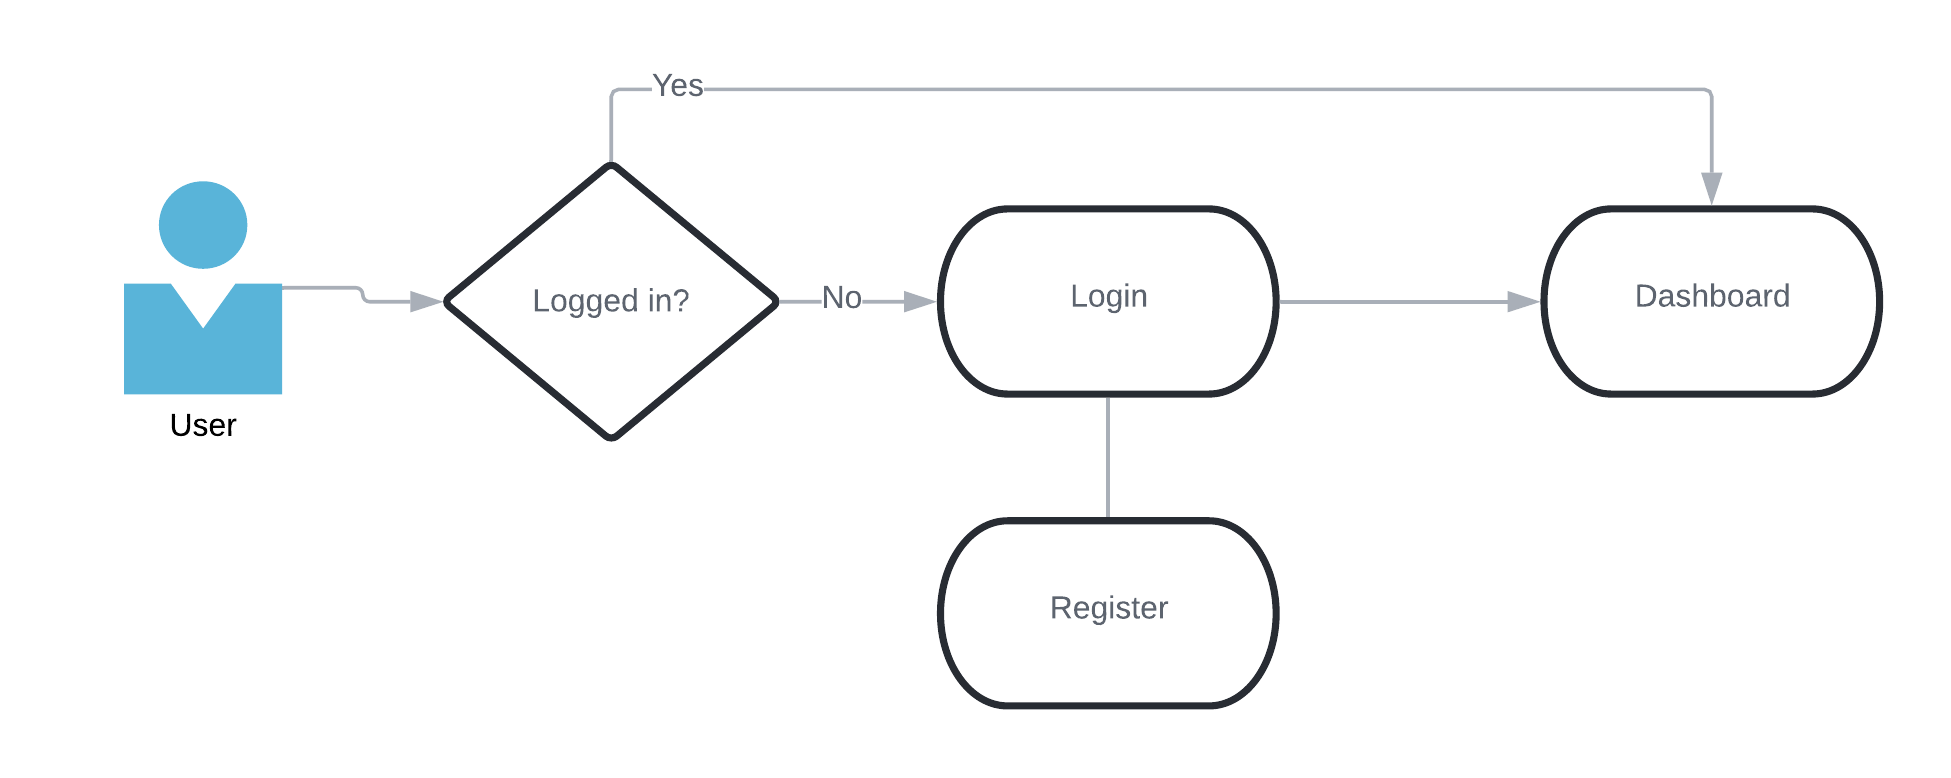
\includegraphics[scale=0.5, width=\textwidth]{figures/images/login_activity.png}
    \caption{Login Activity}
    \label{fig:login_activity_diag}
\end{figure}

Abban az esetben, ha a felhasználó nincs regisztrálva, megteheti ezt a „ Not registered? Click here! ” szövegre kattintva. A regisztrációhoz szükséges egy érvényes e-mail cím, valamint jelszó megadása. Sikeres regisztrálás esetén a felhasználó vissza kerül a bejelentkező ablakra, ahol be tud lépni, azzal a feltétellel, hogy az automatikusan küldött levél által visszaigazolta email címét.

A bejelentkezést követően a felhasználó a főoldalra kerül, ahol a követett termékek listáját tekintheti meg. A listában minden egyes elemnek látható a megnevezése, egy a terméket ábrázoló kép, illetve az adott termék aktuális ára. Továbbá ezen az oldalon lehetősége van a felhasználónak új termékeket hozzá adni a listához, lásd \ref{fig:dashboard_activity_diag} ábra.

\begin{figure}[H]
    \centering
    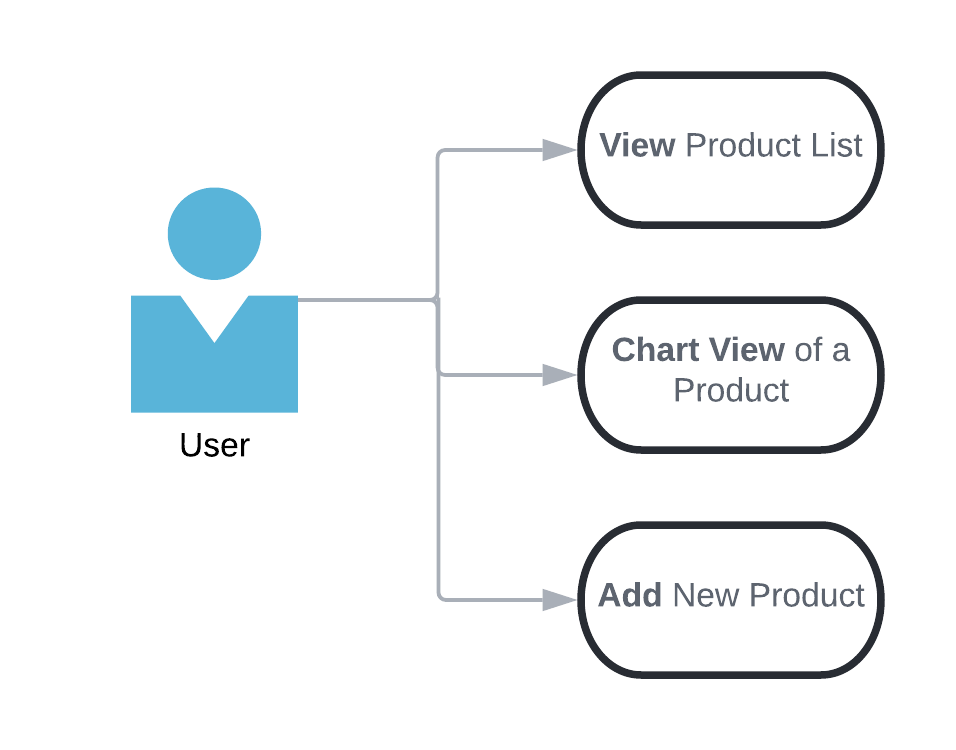
\includegraphics[scale=0.3]{figures/images/dashboard_activity.png}
    \caption{Dashboard Activity}
    \label{fig:dashboard_activity_diag}
\end{figure}

Egy a listában lévő elemre kattintva, az alkalmazás átvisz egy másik oldalra, ahol több információt kapunk a követett termékről. A termék árát tartalmazó gombra kattintva, egy grafikonon tekinthetjük meg a termék árának változását a hozzáadás napjától az aktuális dátumig, lásd \ref{fig:chart_example} ábra. Az „ See product page ” gombra kattintva az alkalmazás megnyitja a terméket tartalmazó weboldalt. Ugyanitt található a törlés gomb, melyre kattintva a termek törlésre kerül a listából és nem fogjuk tovább követni, lásd \ref{fig:detailed_view_diag} ábra.

\begin{figure}[H]
    \centering
    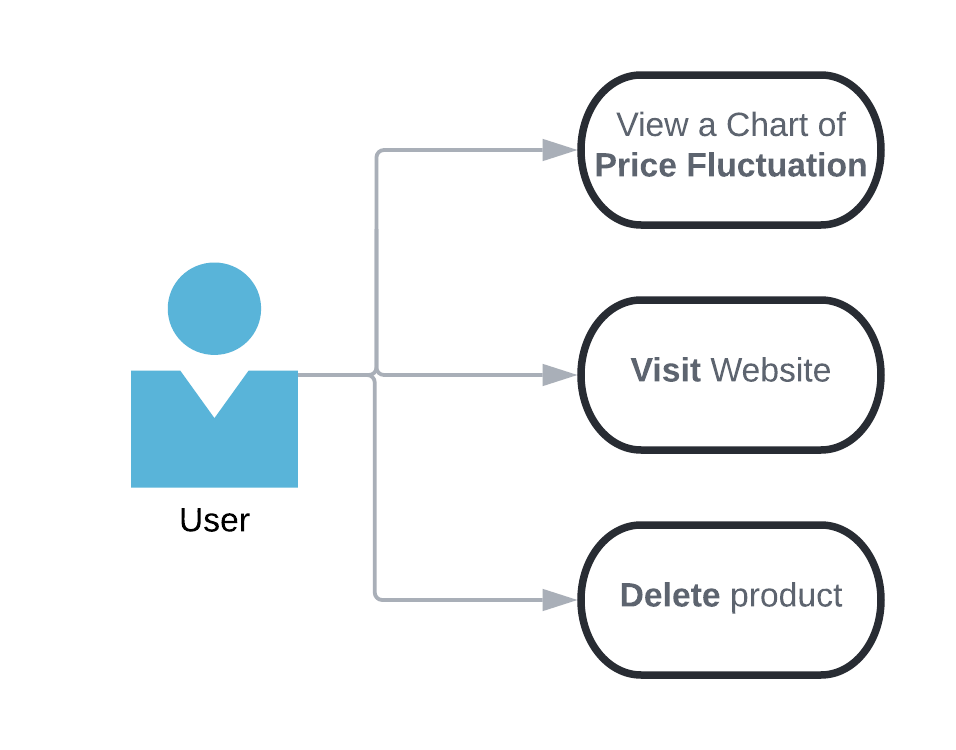
\includegraphics[scale=0.3]{figures/images/chart_view_activity.png}
    \caption{Detailed View}
    \label{fig:detailed_view_diag}
\end{figure}

\begin{figure}[H]
    \centering
    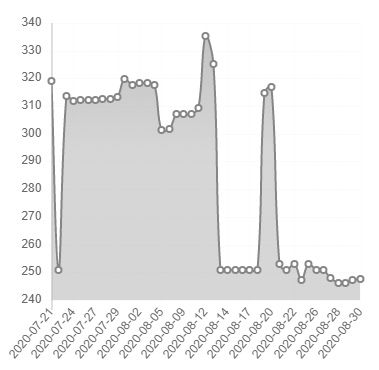
\includegraphics[scale=1]{figures/images/chart_example.png}
    \caption{Chart of Price Change}
    \label{fig:chart_example}
\end{figure}

A felhasználó rendelkezésére áll továbbá két menü. Egy információs, amely röviden leírja az alkalmazás használatát, illetve tartalmazza az általa támogatott weboldalak listáját. A másik a felhasználó fiókjával kapcsolatos információkat és funkciókat tartalmaz. Itt tekintheti meg a felhasználó, hogy milyen email címmel jelentkezett be, megváltoztathatja az aktuális jelszavát, törölheti a fiókját, illetve kijelentkezhet az alkalmazásból, lásd \ref{fig:additional_info} ábra.

\begin{figure}[H]
    \centering
    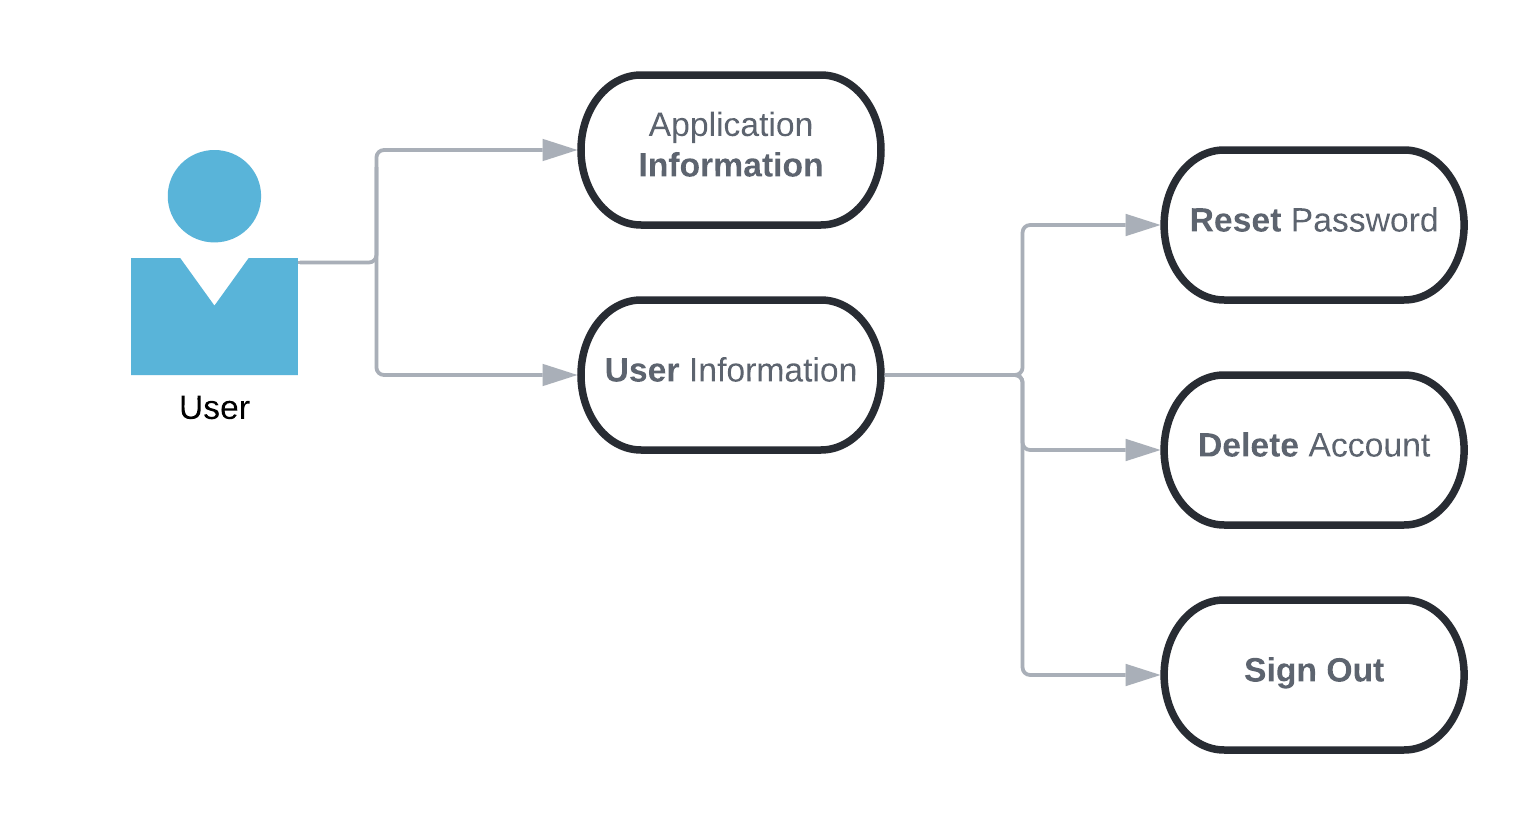
\includegraphics[scale=0.3]{figures/images/additional_features.png}
    \caption{Additional information}
    \label{fig:additional_info}
\end{figure}

\section{Rendszer Követelmények}

\subsection{Funkcionális követelmények}

A rendszernek mindenek elött, egy bejelentkezési, illetve, regisztrálási felülettel kell rendelkeznie. Regisztrálás után, a felhasználónak egy ellenőrző email-t kell kapnia, amivel igazolja, hogy ő a cím tulajdonosa. A bejelentkezés nem lehetséges, abban az esetben, ha a felhasználó nem igazolta vissza az előbb említett email-ben a címét. A cím igazolása egy linkre való kattintással történik.

A felhasználónak lehetősége van a jelszavának módosítására melyet a bejelentkezési felületről ér el. Miután a felhasználó beírta az email címét, egy levelet fog kapni az adott címre, amelyen keresztül új jelszót tud beállítani.

Bejelentkezést követően, a felhasználó egy felületet lát, melyen bizonyos műveleteket végezhet. Megtekintheti a profiljához tartozó email címét, valamint törölheti a felhasználóját. Ugyanakkor, lehetősége van kijelentkezni az alkalmazásából melynek hatására újra a bejelentkezési oldalra kerül.

Ugyancsak a főoldalról a felhasználónak lehetősége van az alkalmazás használatával kapcsolatos információk megtekintésére mely tartalmaz egy listát is. A lista bizonyos weboldalkát tartalmaz, melyeket kiválasztva, az alkalmazás átirányít az adott elem oldalára.

A felhasználónak lehetősége van termékeket hozzáadni és kitörölni a listájából, valamint görgetni a lista tartalmában. A terméklistában egy elemet kiválasztva, részletes reprezentációt kap az adott elem tárolt adatairól.

\subsection{Nem-Funkcionális követelmények}

% TODO
TODO...


%Terv
\chapter{Gyakorlati megvalósítás} \label{chpt:implementation}
\section{Ágensek vezérlése}

\textbf{Hivatkozásra példa}

Az ágensek vezérléséhez a potenciálmező navigációs módszer volt felhasználva. Ez egy bevált módszer a robotrajok vezérléséhez . Az alapötlete, hogy az akadályok taszító erővel hatnak az ágensre és a cél vonzó erővel. Ennek a két erőnek az eredője határozza meg az irányt amerre érdemes haladni.

\subsection{Potenciálmező navigáció}

\textbf{Egyenletekre példa}

A potenciálmező navigációs módszernél az erők nagysága az \eqref{eq:poti} egyenlet szerint van kiszámolva.

\begin{equation}
    \left\{
    \begin{array}{l}
        |\vec{f}_{push}| = a e ^ {- \frac{(x - b_{push}) ^ {2}}{2 c_{push}^2 }} \\
        |\vec{f}_{pull}| = a e ^ {- \frac{(x - b_{pull}) ^ {2}}{2 c_{pull}^2 }} \\
    \end{array}
    \right.
    \label{eq:poti}
\end{equation}

\begin{itemize}
    \item a: Gauss görbe magassága
    \item b: Gauss görbe középpontja
    \item c: Gauss görbe szélessége
\end{itemize}

\begin{equation}
    \vec{f}_{robot} = \sum_{i} \vec{f}_{push_{i}} + \sum_{i} \vec{f}_{pull_{i}}
    \label{eq:poti_eredo}
\end{equation}

Az eredő vektor a \eqref{eq:poti_eredo} képlet szerint volt kiszámolva. 


\chapter{Eredmények}
\section{Cím 1}
Eredmények leírása
\begin{figure}[h]
    \centering
    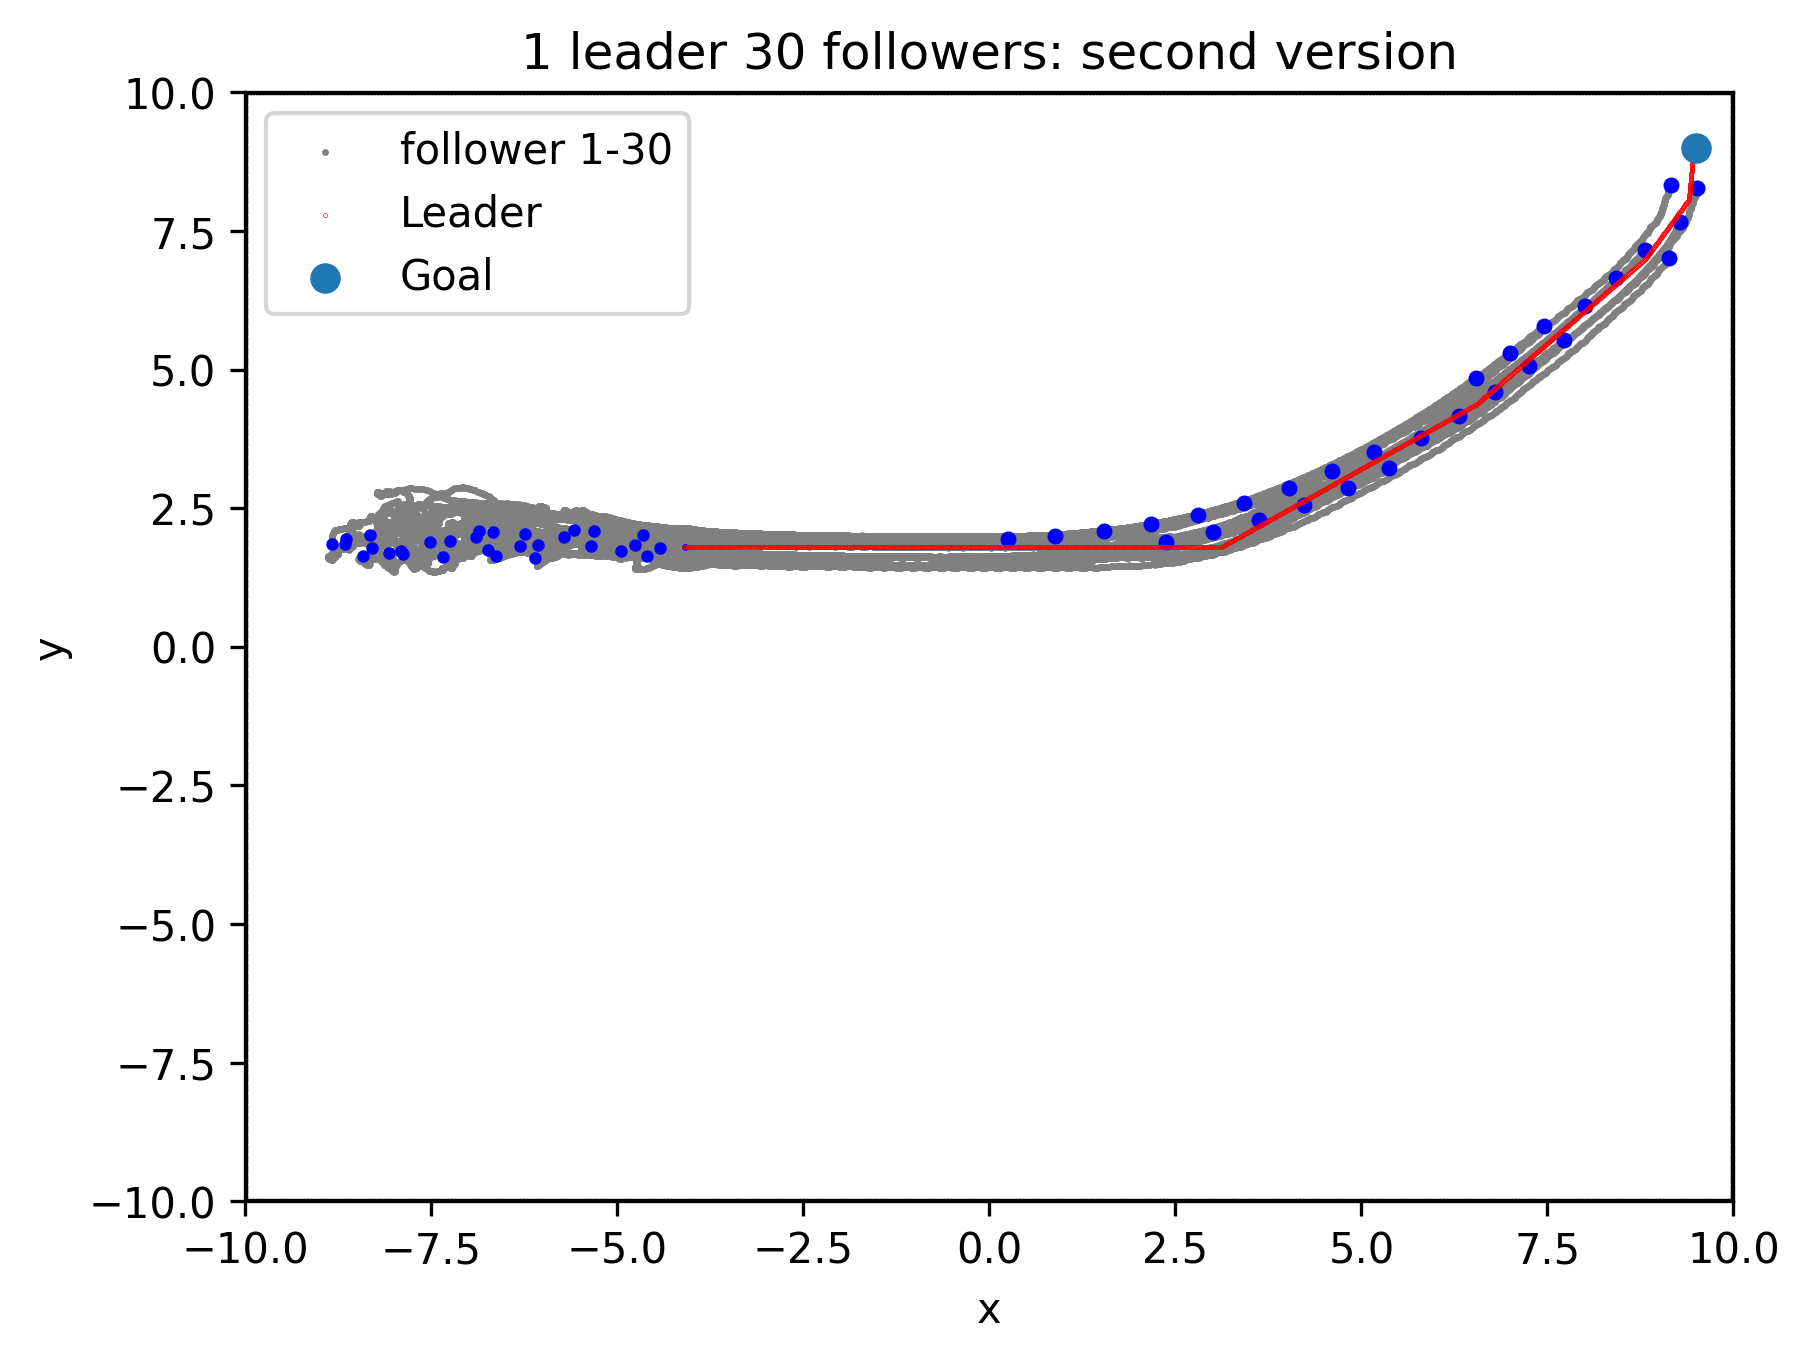
\includegraphics[scale=0.8]{figures/images/results/swarm_second_version.png}
    \caption{30 követő ágens, egy vezér}
    \label{fig:result_30_foll_1_lead}
\end{figure}





%következtetés
\chapter{Összefoglalás}
Röviden összefoglalva a fentebb tárgyaltakat, el lehet mondani, hogy sok esetben megalapozottan ítéljük meg az egyes webáruházakat az árak tudatos manipulálása miatt, viszont mint mindig, ebben az esetben sem lehet általánosítani, hiszen az adatok elemzése során találkoztunk valós kedvezményekkel is, nem csak gyanúsan változó árakkal, melyek félrevezetik vagy egyenesen becsapják a vásárlót. Ezeket figyelembevéve, érdemes mindig több ideig figyelni valamit, ami iránt esetleg vásárlási szándékunk van és nem szabad pusztán az eladóra hagyatkozni, amikor kiírja a termék régi árát, egy nagyobb árleszállítás keretein belül. Erre a célra lett megtervezve és megvalósítva a dolgozatban bemutatott szoftver mely lehetőséget nyújt a felhasználóknak vagy potenciális vásárlóknak automatizálni az esetleges kívánt termékek napi ellenőrzését és az árak összehasonlítását. Mindezt megteheti bárhol is tartózkodik, a megvalósított telefonos alkalmazás segítségével, de egy egyszerűen használható böngészős kiegészítőből is, ha netán inkább az áll közelebb hozzá.

Természetesen egy ilyen típusú alkalmazás fejlesztése folyamatos munkát igényel. Van helye további fejlődésnek, változásnak, optimalizálásnak a jövőre nézve. Mivel a webáruházak struktúrája folyamatosan változik, ezért a háttérben működő szoftvert folyamatosan igazítani kell. Továbbá, egy lehetséges fejlesztés az új webshopok támogatása a jövőben, úgy hazai mint külföldi oldalakat figyelembevéve. Felhasználói felület szintjén is van hely fejlődésnek vagy új akár funkciók hozzáadásának, melyet majd idővel meg is lehet tenni.

\section{Megvalósítások}

A dolgozatban leírtak alapján a következők lettek megvalósítva:
\begin{itemize}
    \item Web Scraping tanulmányozása szakirodalom által
    \item Web Scraping jogi és etikai háttereinek tanulmányozása
    \item Web áruházak struktúrájának tanulmányozása
    \item Az elkészítendő rendszer specifikálása
    \item Firebase adatbázis be üzemelése
    \item Web Scraper implementálása Python script által
    \item Böngésző kiegészítő megvalósítása
    \item Telefonos alkalmazás megvalósítása Flutter segítségével
    \item Admin felület megvalósítása PyQt5 segítségével
    \item Esettanulmány az árak változásáról, külön kitérve a 2020-as Black Friday periódusra
\end{itemize}

\addcontentsline{toc}{chapter}{Irodalomjegyzék}
\bibliographystyle{ieeetr}
\bibliography{References}

%appendix
\appendix
\chapter{Függelék}
\section{Alfejezet}

\subsection{Cím}

\subsubsection{Alcím}




\end{document}